%% LaTeX Beamer presentation template (requires beamer package)
%% see http://bitbucket.org/rivanvx/beamer/wiki/Home
%% idea contributed by H. Turgut Uyar
%% template based on a template by Till Tantau
%% this template is still evolving - it might differ in future releases!

\documentclass{beamer}
\mode<presentation>
{
% 	\usetheme{Singapore}
	\usetheme{Dresden}
	\setbeamertemplate{footline}[frame number]
	\usefonttheme{serif}

	\setbeamertemplate{navigation symbols}{}
    \setbeamertemplate{caption}[numbered]
% 	\setbeamercovered{transparent}
}

\usepackage{cancel}
\usepackage{amsmath}
\usepackage{graphics}

\usepackage{ulem}
\normalem

\usepackage{wasysym}

\usepackage{algorithm}
\usepackage[noend]{algpseudocode}

\title{Algorithm Design, Analysis, and Lower Bound}
\subtitle{--- well, they are just ``divide and conquer'', ``amortized
analysis'', and ``adversary argument'' }

\author{Hengfeng Wei}
\institute{hengxin0912@gmail.com}

\date{\today}

% Delete this, if you do not want the table of contents to pop up at
% the beginning of each subsection:
\AtBeginSubsection[]
{
	\begin{frame}<beamer>
		\frametitle{Outline}
		\tableofcontents[currentsection]
	\end{frame}
}

\AtBeginSection[]
{
	\begin{frame}<beamer>
		\frametitle{Outline}
		\tableofcontents[currentsection]
	\end{frame}
}
% If you wish to uncover everything in a step-wise fashion, uncomment
% the following command:

%\beamerdefaultoverlayspecification{<+->}

\begin{document}

\begin{frame}
	\titlepage
\end{frame}

\begin{frame}
	\frametitle{Outline}
	\tableofcontents
% You might wish to add the option [pausesections]
\end{frame}

%%%%%%%%%%%%%%%%%%%
\section{Divide and Conquer}

\begin{frame}{Recurrences}
%   \[ T(n) = \underbrace{a}_{\# sub-problems}T(\underbrace{n/b}_{\textrm{size of
%   each sub-problem}}) + \underbrace{f(n)}_{\textrm{dividing and combining}}
%   \textrm{ assuming } n = b^{x}
%   \]

  \[
    T(n) = aT(n/b) + f(n), \textrm{ assuming } n = b^{x}
  \]

  \[
    T(n) = \underbrace{\Theta(n^{\log_{b}{a}})}_{\textrm{solving base cases}} +
    \underbrace{\sum_{j = 0}^{\log_{b}{n} - 1} a^{j}
    f(\frac{n}{b^{j}})}_{g(n) = \textrm{dividing and combining}}
  \]

  \begin{description}
    \item[Case 1:] $f(n) = O(n^{\log_{b}{a} - \epsilon}):$ \\
    \hspace{1.0cm} $g(n) = O(n^{\log_{b}{a}}), T(n) = \Theta(n^{\log_{b}{a}})$
    \item[Case 2:] $f(n) = \Theta(n^{\log_{b}{a}}):$  \\
    \hspace{1.0cm} $g(n) = n^{\log_{b}{a}}\log_{b}{n}, T(n) =
    \Theta(n^{\log_{b}{a}})\log_{b}{n}$
    \item[Case 3:] $f(n) = \Omega(n^{\log_{b}{a} + \epsilon}):$ \\
    \hspace{1.0cm} $g(n) = \Theta(f(n)), T(n) = \Theta(f(n))$
  \end{description}
\end{frame}
%%%%%%%%%%%%%
\begin{frame}{Integer Multiplication}
  \begin{exampleblock}{Problem (Integer Multiplication)}
    Multiplying two $n$-bit integers in $o(n^2)$ time. {\small (Assuming $n =
    2^i$.)}
  \end{exampleblock}

  \vspace{0.50cm}

  \begin{columns}
    \column{0.50\textwidth}
      ``Column multiplication in $\Theta(n^2)$''
	  \begin{figure}[htp]
		\begin{center}
		  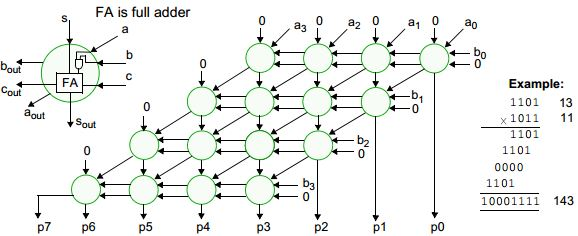
\includegraphics[width = 1.0\textwidth]{figure/bit-multiplication.jpg}
		\end{center}
  	  \end{figure}
    \column{0.50\textwidth}
	  \begin{block}{Elementray operations:}
		\begin{itemize}
		  \item $n$-bit + $n$-bit: $O(n)$
		  \item $1$-bit $\times$ $n$-bit : $O(1)$
		  \item $n$-bit shifted by $1$-bit: $O(1)$
		\end{itemize}
	  \end{block}
  \end{columns}
\end{frame}
%%%%%%%%%%%%%
\begin{frame}{Integer Multiplication}
  \begin{block}{Simple Divide and Conquer:}
  \begin{align*}
    x & = x_L : x_R = 2^{n/2} x_L + x_R  \\
    y & = y_L : y_R = 2^{n/2} y_L + y_R
  \end{align*}

  \begin{align*}
    xy & = (2^{n/2} x_L + x_R) (2^{n/2} y_L + y_R) \\
       & = 2^{n} x_L y_L + 2^{n/2} (x_L y_R + x_R y_L) + x_R y_R
  \end{align*}

  \[
    T(n) = 4T(n/2) + \Theta(n) = \Theta(n^2)
  \]
  \end{block}
\end{frame}
%%%%%%%%%%%%%
\begin{frame}{Integer Multiplication}
  \begin{block}{A Little History:}
  \begin{itemize}
    \item Kolmogorov (1952) conjecture: $\Omega(n^2)$
    \item Kolmogorov (1960) seminar
    \item Karatsuba (23 Y/O., \emph{within a week}): $\Theta(n^{1.59})$
    \item ``The Complexity of Computations'' (1995)
  \end{itemize}
  \end{block}
\end{frame}
%%%%%%%%%%%%%
\begin{frame}{Integer Multiplication}
  \begin{block}{Karatsuba Algorithm:}
    \[
      T(n) = 3T(n/2) + \Theta(n) = \Theta(n^{\log_{2}{3}}) = \Theta(n^{1.59})
    \]

    \[
      \underbrace{(x_L + x_R) (y_L + y_R)}_{P_0} = \underbrace{x_L y_L}_{P_1} +
      (x_L y_R + x_R y_L) + \underbrace{x_R y_R}_{P_2}
    \]

    \[
      xy = 2^{n} P_1 + 2^{n/2} (P_0 - P_1 - P_2) + P_2
    \]
  \end{block}
\end{frame}
%%%%%%%%%%%%%
\begin{frame}{Matrix Multiplication}
  \begin{exampleblock}{Problem (Matrix Multiplication)}
    Multiplying two $n \times n$ matrices in $o(n^3)$ time. {\small (Assuming $n
    = 2^i$.)}
    \[ Z = X \times Y \]
  \end{exampleblock}

  \vspace{0.50cm}
  \begin{columns}
    \column{0.40\textwidth}
	  \[ Z_{ij} \]

	  \[ T(n) = \Theta(n^2 \cdot n) = \Theta(n^3) \]
    \column{0.60\textwidth}
	  \begin{block}{Elementrary operations:}
	    \begin{itemize}
	      \item integer addition: $O(1)$
	      \item integer multiplication: $O(1)$
	    \end{itemize}
	  \end{block}
  \end{columns}
\end{frame}
%%%%%%%%%%%%%
\begin{frame}{Matrix Multiplication}
  \begin{displaymath}
	X = \begin{bmatrix} A & B \\ C & D \end{bmatrix}, \quad
	Y = \begin{bmatrix} E & F \\ G & H \end{bmatrix} \qquad (A \ldots H \in
	\mathbb{R}^{n/2} \times \mathbb{R}^{n/2})
  \end{displaymath}

  \[
    XY = \begin{bmatrix} AE + BG & AF + BH \\ CE + DG & CF + DH \end{bmatrix}
  \]

  \[
    T(n) = 8T(n/2) + \Theta(n^2) = \Theta(n^3)
  \]
\end{frame}
%%%%%%%%%%%%%
\begin{frame}{Matrix Multiplication}
  \begin{block}{Strassen Algorithm:}
    \[
      T(n) = 7T(n/2) + \Theta(n^2) = \Theta(n^{\lg {7}}) =
     \Theta(n^{2.808})
    \]
  \end{block}

  \begin{itemize}
    \item Strassen (1969): $\Theta(n^{2.808})$
    \item (2014): $\Theta(n^{2.373})$
    \item Known lower bound: $\Omega(n^{2})$
  \end{itemize}
\end{frame}
%%%%%%%%%%%%%
\begin{frame}{Computing $\lceil \sqrt{N} \rceil$}
  \begin{exampleblock}{Problem (Computing $\lceil \sqrt{N} \rceil$)}
    Given an $n$-bit natural number $N$, how to compute $\lceil \sqrt{N} \rceil$
    using only $O(n)$ additions and shifts?
  \end{exampleblock}

  \vspace{0.50cm}
  \begin{columns}
    \column{0.55\textwidth}
	  \begin{block}{Elementrary operations:}
	    \begin{itemize}
	      \item $n$-bit + $n$-bit: $O(1)$
	      \item $n$-bit shifted by $1$-bit: $O(1)$
	      \item $\Rightarrow x^2: O(n)$
	    \end{itemize}
	  \end{block}
	\column{0.45\textwidth}
	  \begin{itemize}
	    \item Na{\"i}ve search: $O(2^{n} \cdot n)$
	    \item Binary search: $O(n \cdot n)$
	    \item Binary search in range:
	    \[
	      2^{\lfloor \frac{n-1}{2} \rfloor} \le \lceil \sqrt{N} \rceil \le
	      2^{\lceil \frac{n}{2} \rceil}
	    \]
	    \[
	      \lg{(2^{\lceil \frac{n}{2} \rceil} - 2^{\lfloor
	      \frac{n-1}{2} \rfloor})} = n
	    \]
	    \[ O(n \cdot n) \]
	  \end{itemize}
  \end{columns}
\end{frame}
%%%%%%%%%%%%%
\begin{frame}{Computing $\lceil \sqrt{N} \rceil$}
  \begin{block}{A Little History:}
    \begin{itemize}
      \item Mid-term problem ($\sim 2008$)
      \item ($\sim$ 2013): $O(n^2)$
      \item (2014): $O(n)$
    \end{itemize}
  \end{block}
\end{frame}
%%%%%%%%%%%%%
\begin{frame}{Computing $\lceil \sqrt{N} \rceil$}
  Given
  \[ M = \lfloor N/4 \rfloor, x = \lceil \sqrt{M} \rceil,
    \textrm{ and } (x, x^2),
  \]
  what is
  \[ y = \lceil \sqrt{N} \rceil \textrm{ and } (y, y^2)? \]

%   \begin{itemize}
%     \item $N = 280 \quad y = \lceil \sqrt{280} \rceil = 17 \quad y^2 = 289$
%     \item $M = \lfloor 280/4 \rfloor = 70 \quad x = \lceil \sqrt{70} \rceil =
%     9 \quad x^2 = 81$
%   \end{itemize}
  \begin{exampleblock}{An Example:}
  \[
  \begin{array}{lll}
    N = 280 & y = \lceil \sqrt{280} \rceil = 17 & y^2 = 289 \\
    M = \lfloor 280/4 \rfloor = 70 & x = \lceil \sqrt{70} \rceil = 9 & x^2 = 81
    \\
    M = \lfloor 70/4 \rfloor = 17 & x = \lceil \sqrt{17} \rceil = 5 & x^2 = 25
    \\
    M = \lfloor 17/4 \rfloor = 4 & x = \lceil \sqrt{4} \rceil = 2 & x^2 = 4
    \\
    M = \lfloor 4/4 \rfloor = 1 & x = \lceil \sqrt{1} \rceil = 1 & x^2 = 1
  \end{array}
  \]
  \end{exampleblock}
\end{frame}
%%%%%%%%%%%%%
\begin{frame}{Computing $\lceil \sqrt{N} \rceil$}
  \begin{algorithm}[H]
    \caption{Computing $\lceil \sqrt{N} \rceil$.}
    \begin{algorithmic}[]
      \Procedure{Sqrt-Root}{$N$}
	    \If{$N < 3$}
	      \State \Return $1 \Rightarrow (1,1); 2 \Rightarrow (2,4); 3 \Rightarrow
	    (2,4)$
	    \EndIf
	    \State $M \gets \lfloor N/4 \rfloor$
	    \State $(x, x^2) \gets \textsc{Sqrt-Root}{(M)}$
		\State \Return the $(y, y^2)$ with $y^2 \sim N$:
           \[
			(y, y^2) = \left\{ \begin{array}{ll}
			y = 2x & y^2 = 4x^2 \\
			y = 2x + 1 & y^2 = 4x^2 + 4x + 1 \\
			y = 2x - 1 & y^2 = 4x^2 - 4x + 1
			\end{array} \right.
	      \]
	  \EndProcedure
    \end{algorithmic}
  \end{algorithm}
\end{frame}
%%%%%%%%%%%%%
\begin{frame}{Computing $\lceil \sqrt{N} \rceil$}
  \[ \xout{T(n) = T(n/4) + O(1) = \Theta(\lg n)} \]

  \[ T(n) = T(n - 2) + O(1) = \Theta(n) \]
\end{frame}
%%%%%%%%%%%%%
\begin{frame}{VLSI Layout}
  \begin{exampleblock}{Problem (Area-Efficient VLSI Layout)}
    Embedding a complete binary tree with $n$ leaves into a grid with minimum
    area.
    \begin{itemize}
      \item VLSI: Very Large Scale Integration
      \item complete binary tree circuit of $\#layer = 3,5,7,\ldots$
%       \item $n$ leaves (\textcolor{red}{why only leaves?})
      \item vertex on grid; no crossing edges
      \item area = width $\times$ height
    \end{itemize}
  \end{exampleblock}
\end{frame}
%%%%%%%%%%%%%
\begin{frame}
  \frametitle{VLSI Layout}

  \begin{itemize}
    \setlength{\itemsep}{0.50cm}
    \item Na\"{\i}ve embedding
     \[ H(n) = H(\frac{n}{2}) + \Theta(1) = \Theta(\lg n) \]
     \[ W(n) = 2W(\frac{n}{2}) + \Theta(1) = \Theta(n) \]
     \[ A(n) = \Theta(n \lg n) \]
    \item Smart (H-Layout) embedding
    \[ \Box \times \Box = n? \; 1 \times n;\; \frac{n}{\lg n} \times \lg n;\;
    \textcolor{blue}{\sqrt{n} \times \sqrt{n}}
    \]
    Goal: $H(n) = \Theta(\sqrt{n}); W(n) = \Theta(\sqrt{n}); A(n) = \Theta(n).$
    \[
      H(n) = \Box H(\frac{n}{\Box}) + O(\Box); H(n) = 2 H(\frac{n}{4}) +
      O(n^{\frac{1}{2} - \epsilon})
    \]
    \[ H(n) = 2H(\frac{n}{4}) + \Theta(1) \]
    \centering \textcolor{blue}{Here it is: H-Layout}
  \end{itemize}
\end{frame}
%%%%%%%%%%%%%
\begin{frame}{VLSI Layout}
  \begin{figure}[htp]
	\begin{center}
	  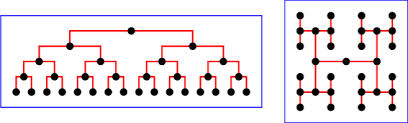
\includegraphics[width = 0.80\textwidth]{figure/vlsi}
	\end{center}
  \end{figure}
\end{frame}
%%%%%%%%%%%%%
\begin{frame}{Local Minimum in Tree (Optional)}
  \begin{exampleblock}{Problem (Local Minimum in Tree)}
    Consider an $n$ node complete binary tree $T$. Each node $v$ is labeled with
    a (distinct) number $x_v$, how to find a \emph{local minimum} in $O(\log n)$
    time?
  \end{exampleblock}
\end{frame}
%%%%%%%%%%%%%
\begin{frame}{Local Minimum in Grid (Optional)}
  \begin{exampleblock}{Problem (Local Minimum in Grid)}
    Consider an $n \times n$ grid. Each cell is labeled with a (distinct) number
    and has (at most) four neighbors. How to find a \emph{local minimum} in
    $O(n)$ time?
  \end{exampleblock}
\end{frame}
%%%%%%%%%%%%%%%%%%%
\section{Amortized Analysis}

%%%%%%%%%%%%%
\begin{frame}{Amortized Analysis}
  \begin{quote}
    Amortized analysis is a strategy for analyzing \\
    \textcolor{blue}{a sequence of operations} \textcolor{purple}{irrespective
    of the input} \\ to show that
    \textcolor{blue}{the average cost per operation} is small, \\
    even though a \textcolor{blue}{single operation within the sequence might be
    expensive}.
  \end{quote}

  \vspace{0.30cm}
  Key points:

  {\small (Array doubling; Multipop stack; Binary counter; Stack $\rightarrow$
  Queue)}
  \begin{itemize}
    \setlength{\itemsep}{3pt}
    \item cheap ops (often) vs. expensive ops (rare)
    \item on op sequence \textcolor{red}{(where?)}; not on separate ops
    \item $\neq$ average-case analysis; \textcolor{purple}{no probability
    here}\\
    (\textsc{Quick-Sort}, \textsc{HashTable})
    \item worst-case analysis; upper-bound
  \end{itemize}
\end{frame}
%%%%%%%%%%%%%
\begin{frame}{Methods for Amortized Analysis}
  \begin{enumerate}
    \setlength{\itemsep}{0.30cm}
    \item Summation Method
      \begin{itemize}
        \item $\sum_{i = 1}^{n} c_i / n$
        \item the op. sequence is known and easy to analyze (pattern)
      \end{itemize}
    \item Accounting Method
	  \begin{itemize}
		\setlength{\itemsep}{0.15cm}
	    \item impose an extra charge on inexpense ops and use it to pay for
	    expensive ops later on
	    \item $\hat{c_i} = c_i + a_i \; (a_i >=< 0)$ \\ (amortized cost = actual
	    cost + accounting cost)
	    \item $\forall n, \sum_{i=1}^{n} \hat{c_i} = \sum_{i=1}^{n} c_i +
	    \sum_{i=1}^{n} a_i$
	    \item $\forall n, \sum_{i=1}^{n} \hat{c_i} \geq \sum_{i=1}^{n} c_i
	    \Rightarrow \textcolor{blue}{\forall n, \sum_{i=1}^{n} a_i \geq 0}$
	    \item put the accounting cost on specific objects
	  \end{itemize}
    \item \textcolor{gray}{Potential Method}
	  \begin{itemize}
	    \item see Section 17.3 of CLRS (3rd edition)
	  \end{itemize}
  \end{enumerate}
\end{frame}
%%%%%%%%%%%%%
\begin{frame}{Array Doubling Revisited}
  \begin{block}{Summation Method:}
    \emph{on any sequence of $n$ \textsc{Insert} ops on an initially empty
    array}

  \vspace{0.30cm}
  Q: What is the cost of $c_i$ of the $i$-th op?
  \[
    \begin{array}{cccccccccccc}
      i: 	& 0 & 1 & 2 & 3 & 4 & 5 & 6 & 7 & 8 & 9 & 10 \\
      c_i:  &   & 1 & 2 & 3 & 1 & 5 & 1 & 1 & 1 & 8 & 1  \\
    \end{array}
  \]

	\begin{displaymath}
	  c_i = \left\{ \begin{array}{ll}
	    (i-1)+1 = i & \textrm{if $i - 1$ is an exact power of 2}\\
	    1 & \textrm{o.w.}
	  \end{array} \right.
	\end{displaymath}

  \[
	\sum_{i=1}^{n} c_i \le n + \sum_{j=0}^{\lceil \lg n \rceil - 1} 2^{j} = n +
	(2^{\lceil \lg n \rceil} - 1) \le n + 2n = 3n
  \]

  The \emph{amortized} cost of a single operation is 3.
  \end{block}
\end{frame}
%%%%%%%%%%%%%
\begin{frame}{Array Doubling Revisited}
  \begin{block}{Accounting method:}
	\[ \hat{c_i} = 3 \]
	\[ \textrm{Why not } \hat{c_i} = 2 ?\]

    An example:
    \[ 0;0;0;0;1 \Rightarrow 0;0;0;0;1;1;1;1 \Rightarrow \frownie{} \]

	\[
	  \hat{c_i} = 3 = \underbrace{1}_{\textrm{insert}} +
	  \underbrace{1}_{\textrm{move itself}} + \underbrace{1}_{\textrm{move another}}
	\]

  \begin{table}
    \begin{tabular}{c|ccc}
	  & $\hat{c_i}$ & $c_i$ (actual cost) & $a_i$ (accounting cost)
	  \\ \hline
	  \textsc{Insert}(normal) & 3 & 1 & 2 \\
	  \textsc{Insert}(expensive) & 3 & 1 + t & -t + 2
    \end{tabular}
  \end{table}

  \end{block}
\end{frame}
%%%%%%%%%%%%%
\begin{frame}{Two Stacks, One Queue}

  \begin{exampleblock}{Problem (Two Stacks, One Queue)}
    Correctness proof

    Amortized analysis
  \end{exampleblock}

  \begin{algorithm}[H]
    \caption{Simulating a queue using two stacks $S_1, S_2$.}
    \begin{algorithmic}[]
      \Procedure{Enq}{$x$}
		\State \textsl{Push}($S_1, x$)
      \EndProcedure

	  \Statex

      \Procedure{Deq}{\null}
        \If{$S_2 = \emptyset$}
          \While{$S_1 \neq \emptyset$}
            \State \textsl{Push}($S_2$, \textsl{Pop}($S_1$))
          \EndWhile
        \EndIf
        \textsl{Pop}($S_2$)
      \EndProcedure
    \end{algorithmic}
  \end{algorithm}

  Ex: \textsc{Enq}$(1,2,3)$, \textsc{Deq}$()$, \textsc{Deq}$()$,
  \textsc{Enq}$(4)$, \textsc{Deq}$()$
\end{frame}
%%%%%%%%%%%%%
\begin{frame}{Two Stacks, One Queue}
  \begin{center}
    Simple observation: \fbox{$S_1$ to push; $S_2$ to pop.}
  \end{center}

  \begin{block}{Correctness proof:}
    \[
      \textrm{FIFO:} \quad \textsc{Deq}() = x \prec \textsc{Deq}() = y
      \quad \textcolor{blue}{\Rightarrow} \quad Enq(x) \prec \textsc{Enq}(y)
    \]
  \end{block}

  \begin{itemize}
    \item Summation method: the sequence is \uppercase{not} known
    \item Accounting method: $\hat{c_i} = c_i + a_i$
    \[ \forall n, \sum_{i}^{n} a_i \geq 0 \]
  \end{itemize}
\end{frame}
%%%%%%%%%%%%%
\begin{frame}{Two Stacks, One Queue}
  \begin{table}
    \begin{tabular}{ccccc}
	  item: & \textsc{Push} into $S_1$ & \textsc{Pop} from $S_1$ & \textsc{Push}
	  into $S_2$ & \textsc{Pop} from $S_2$ \\
	  & \underbrace{1}_{\textsc{Enq}} & 1 & 1 & \underbrace{1 +
	  1}_{\textsc{Deq}(normal)}
    \end{tabular}
  \end{table}

  $\#S_1 = t:$
  \begin{table}
    \begin{tabular}{c|ccc}
	  & $\hat{c_i}$ & $c_i$ (actual cost) & $a_i$ (accounting cost)
	  \\
	  \textsc{Enqueue} & 3 & 1 & 2 \\
	  \textsc{Dequeue}(normal) & 2 & 2 & 0 \\
	  \textsc{Dequeue}(expensive) & 2 & 2+2t & -2t
    \end{tabular}
  \end{table}

  \[ \sum_{i=1}^{n} a_i = \#S_1 \times 2 \geq 0 \]
\end{frame}
%%%%%%%%%%%%%%%%%%%
\section{Adversary Argument}

%%%%%%%%%%%%%
\begin{frame}{Lower Bound}
  \[ T(A) = \max_{I} T(A,I) \]

  \[ T(P) = \min_{A} \max_{I} T(A,I) \]

  \[
    UB(P) = t \iff \exists_{A} T(A) \le t \iff \exists_{A} \forall_{I} T(A, I)
    \le t
  \]

  \[
    LB(P) = t \iff \forall_{A} T(A) \geq t \iff \forall_{A} \exists_{I} T(A, I)
    \geq t
  \]
\end{frame}
%%%%%%%%%%%%%
\begin{frame}{Lower Bound}
  \begin{align*}
    n! & \Rightarrow n^2 \textrm{ \it (playing card)} \\
       & \Rightarrow n \lg n \textrm{ \it (MergeSort by John von Neumann@1948)}
       \\
       & \textcolor{blue}{\textrm{\textsc{Sorting}}} \\
       & \Leftarrow n \lg n \textrm{ \it (decision tree)} \\
       & \Leftarrow n
  \end{align*}

  \begin{columns}
    \column{0.50\textwidth}
	  \begin{align*}
	    n^2 & \Rightarrow n \lg n \Rightarrow n \\
	        & \textcolor{blue}{\textsc{Median} (k^{th})} \\
	        & \Leftarrow n
	  \end{align*}
    \column{0.50\textwidth}
	  \begin{align*}
	    & \Rightarrow 16n \textrm{ \it (median-of-median)} \\
	    & \Rightarrow 2.95n \textrm{ \it ()}  \\
	    & \textcolor{blue}{\textsc{Median} (k^{th})} \\
	    & \Leftarrow \frac{3n}{2} - \frac{3}{2}
	  \end{align*}
  \end{columns}

  \begin{center}
    ``Time Bounds for Selection'' \textbf{BFPRT}@1973
  \end{center}
\end{frame}
%%%%%%%%%%%%%
\begin{frame}{Matrix Search}
  \begin{exampleblock}{Problem (Matrix Search)}
  	Given an $n \times n$ integer matrix with both rows and columns in increasing
  	order, how to find an element $x$ in $O(n)$ time?

	\vspace{0.20cm}

  	Give an adversary argument to establish its lower bound.
  \end{exampleblock}

	  \begin{figure}[htp]
	    \begin{center}
	      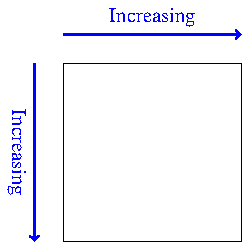
\includegraphics[width = 0.25\textwidth]{figure/increasing-matrix.pdf}
	    \end{center}
	  \end{figure}
\end{frame}
%%%%%%%%%%%%%
\begin{frame}{Matrix Search}
  Finding $x = 28$:
  \begin{table}
	\begin{tabular}{|c|c|c|c|c|}
	  \hline
	  1 	& 3 	& 5 	& 7 	& 9 	\\ \hline
	  6 	& 8 	& 12 	& 14 	& 15  	\\ \hline
	  10 	& 13 	& 18 	& 22 	& 33  	\\ \hline
	  20 	& 24 	& 29 	& 30 	& 35 	\\ \hline
	  26 	& 31 	& 32 	& 40 	& 45 	\\ \hline
	\end{tabular}
  \end{table}

  Algorithm:
  \begin{enumerate}
    \item check the lower left element
    \item delete a row or a column; goto \textcolor{blue!80}{1}.
  \end{enumerate}

  \[ T(n) = 2(n-1) + 1 = 2n - 1 = \Theta(n) \]
\end{frame}
%%%%%%%%%%%%%
\begin{frame}{Matrix Search}
  Adversary argument:
  \[
    LB(P) = t \iff \forall_{A} T(A) \geq t \iff \forall_{A} \exists_{I} T(A, I)
    \geq t
  \]

  \textcolor{blue}{Adversary} is constructing an input:
  \begin{table}
	\begin{tabular}{|c|c|c|c|c|}
	  \hline
	  1 	& 3 	& 5 	& 7 	& $\ast$ 	\\ \hline
	  6 	& 8 	& 12 	& \textcolor{red}{$\ast$(14)}	& $\ast$  	\\ \hline
	  10 	& 13 	& $\ast$	& $\ast$ 	& 33  	\\ \hline
	  20 	& $\ast$ 	& \textcolor{blue}{$\ast$(29)} 	& 30 	& 35 	\\ \hline
	  $\ast$ 	& \textcolor{blue}{$\ast$(31)}	& 32 	& 40 	& 45 	\\ \hline
	\end{tabular}
  \end{table}

  \begin{description}
    \item[$i + j \le n:$] $M[i][j] < n$
    \item[$i + j > n:$] $M[i][j] > n$
  \end{description}

  To prove: all the elements on the two diagonals must be checked
\end{frame}
% \begin{frame}
%   \frametitle{01 Adversary}
%
%   \begin{Problem}[01 Adversary $\lbrack {\bf P_{245}, 5.20} \rbrack$]
%     bit array $A[1 \ldots n]$; if it contains the substring $01$? \\
%     can we answer this question without looking at every bit?
%   \end{Problem}
%
%   \begin{itemize}
%     \item $n$ is odd ($n=9$): check each \emph{even} bit $A[2], A[4], \ldots
%     A[8]$
%       \begin{itemize}
%         \item all 1: $A[n]$
%         \item all 0: $A[1]$
%         \item all 1 come before 0 (1\;1\;0\;0): $A[4], A[6]$
%         \item $\exists i < j, A[i] = 0, A[j] = 1\; (A[2], A[6])$
%       \end{itemize}
%     \item $n$ is even
%       \begin{itemize}
%         \item $1\;1\;1\;1\;1\;1\; \Box \Box \Box \Box \Box \Box\; 0\;0\;0\;0$
%         \item Init: $l = 0; r = n + 1$
%         \item Invariant: $r - l - 1$ is even
%         \item \textsc{Look($i$):} $i \leq l \Rightarrow 1$; $i \geq r
%         \Rightarrow 0$; \\
%         $i-r$ is even $\Rightarrow (r \gets i; 0)$; \\
%         $i-l$ is even $\Rightarrow (l \gets i; 1)$
%       \end{itemize}
%   \end{itemize}
% \end{frame}
% %%%%%%%%%%%%%%%%%%%
\section*{Summary}
\begin{frame}{}
  \begin{figure}[htp]
    \begin{center}
      
\includegraphics[width=0.618\textwidth]{figure/thankyou.jpg}
    \end{center}
  \end{figure}
\end{frame}
%%%%%%%%%%
\end{document}
